\documentclass[main.tex]{subfiles}
\begin{document}

\textbf{Group 1} Design a Keplerian Beam expander (explain the difference and the advantages)\\

\begin{figure}\label{fig:1}
\centering\fbox{\includegraphics[height=2.0in]{figures/setup2/Keplerian-Beam-Expander.png}}
\caption{Keplerian Beam Expander Schematic}
\end{figure}

\begin{equation}\label{eq:e1}
M=f_2/f_1= R_2/R_1 = h2_1
\end{equation}

In the Keplerian model the focal lengths of both lenses will be positive,their addition resulting in a focal point in the gap between the lenses at the point where the two focal lengths meet. Because there is a high power density due to the focused spot size at the focal point between the lenses, keplerian beam expanders are not recommended for use with lasers with high pulse energies. This is because the high pulse energy density at the focal point can cause the air to arc. However, if you would like to clean up the beam as it passes through the beam expander, this focal point can be a handy palce to position a pinhole. It will be necessary to make certian that the energy density of the ebam at the focal point does not exceed the damage threshold limitation of the pinhole material. Also, in imaging applications, because the image will be inverted and reverted at the output, the addition of a third lens (relay lens) may be required to correct the image orientation.\\

\textbf{Q&A} Describe your approach for building the system and its functionality.\\

\textbf{Q&A} After designing the optical system send to me a Bill of Costs including lenses (specifying type), beam splitters, mirrors, posts, holders, cages, stages. https://www.thorlabs.com/\\

\textbf{Specs Group 1-2} The system is not affected by chromatic aberration, the beam size has to be adjustable according to tunable focusing, Initial beam size of the laser $\SI{2}{m\metre}$.\\

Laser beam $d=2mm$, Camera Sensor $1/1.8$, and has to sense variation of the refractive index in the \SI{20}{m\second} regime. (specs on the sensor side)\\

\begin{figure}\label{fig:2}
\centering\fbox{\includegraphics[height=2.0in]{figures/setup2/comsol/comsol_1.png}}
\caption{COMSOL Multiphysics Simulation of Keplerian Beam Expander}
\end{figure}

Attached page contains possible combinations of lenses for purchase from Newport Photonics.


\begin{figure}\label{fig:3}
\centering\fbox{\includegraphics[width=2.5in]{figures/setup1/Zbeam_1.jpeg}}
\centering\fbox{\includegraphics[width=2.5in]{figures/setup1/Zbeam_2.jpeg}}
\caption{Set up 1, Aperture stop at varying distances while maintaining centered beam path.}
\end{figure}

\begin{figure}\label{fig:4}
\centering\fbox{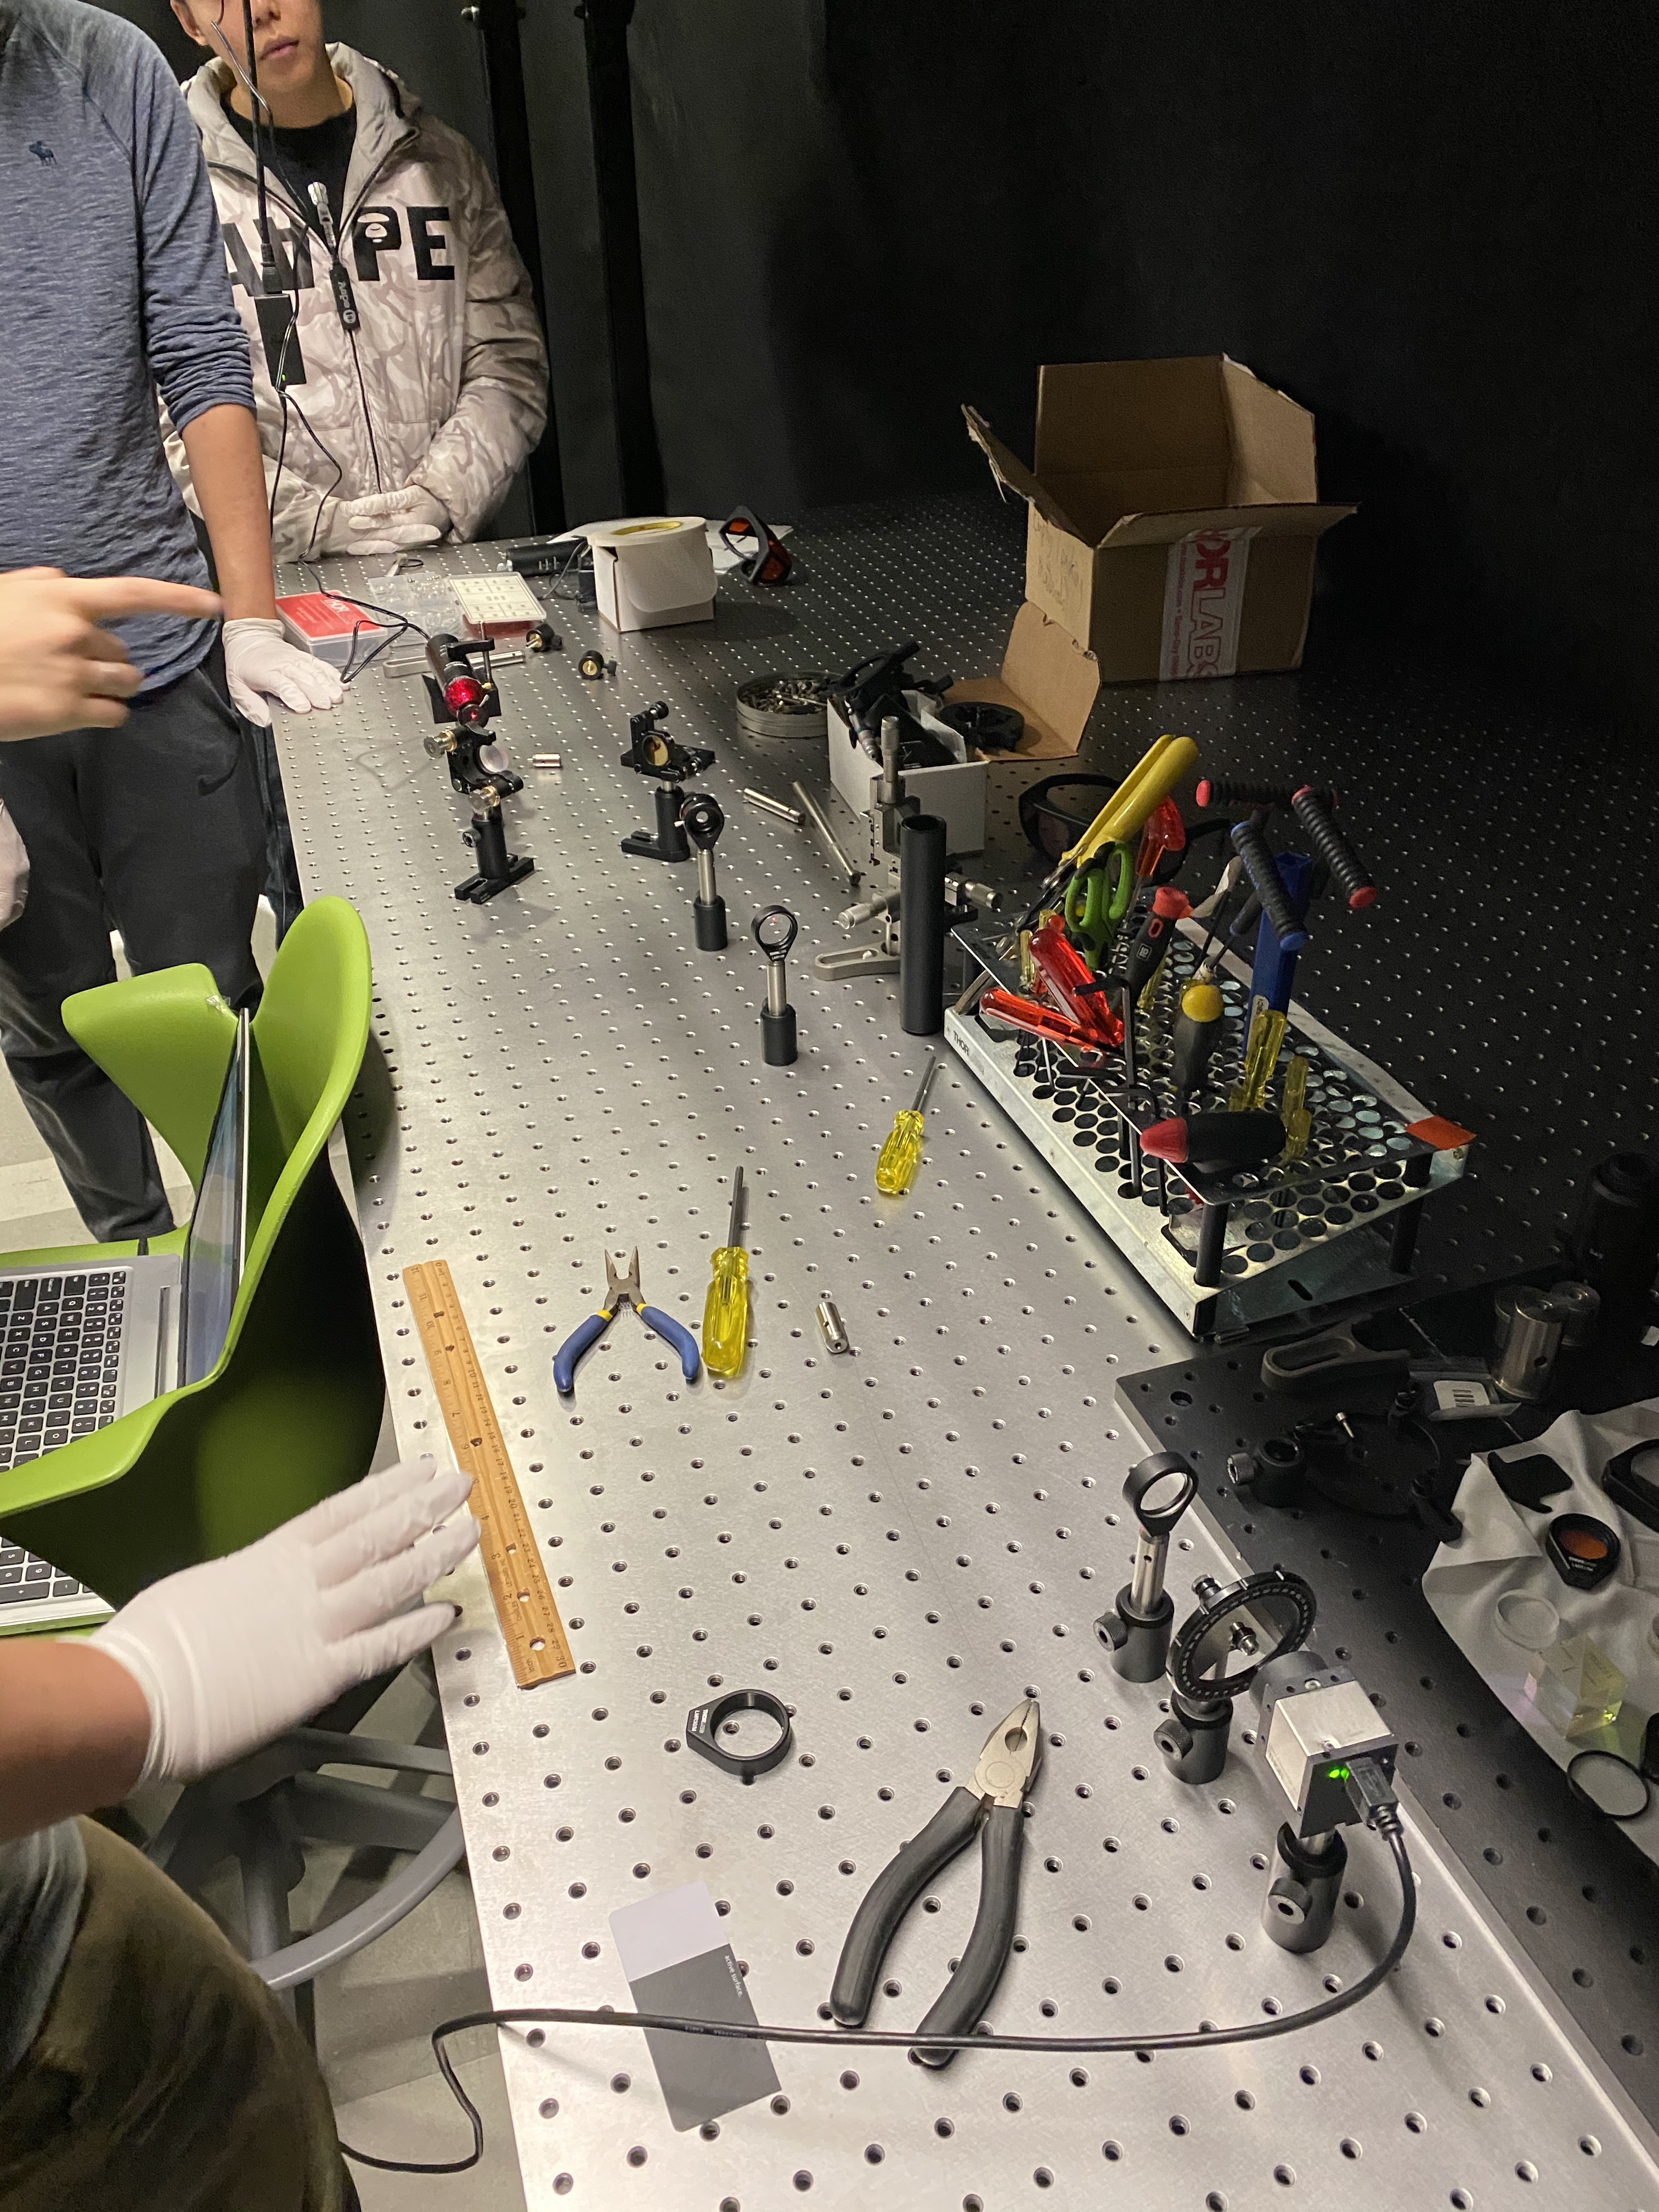
\includegraphics[width=2.5in]{figures/setup2/Keplerian_1.png}}
\caption{Setup 2, Keplerian beam expander with $f_1 = \SI{100}{m\metre}$ \& $f_2=\SI{400}{m\mete}$ focal lengths of two Bi-Convex lenses.}
\end{figure}

\begin{figure}\label{fig:5}
\centering\fbox{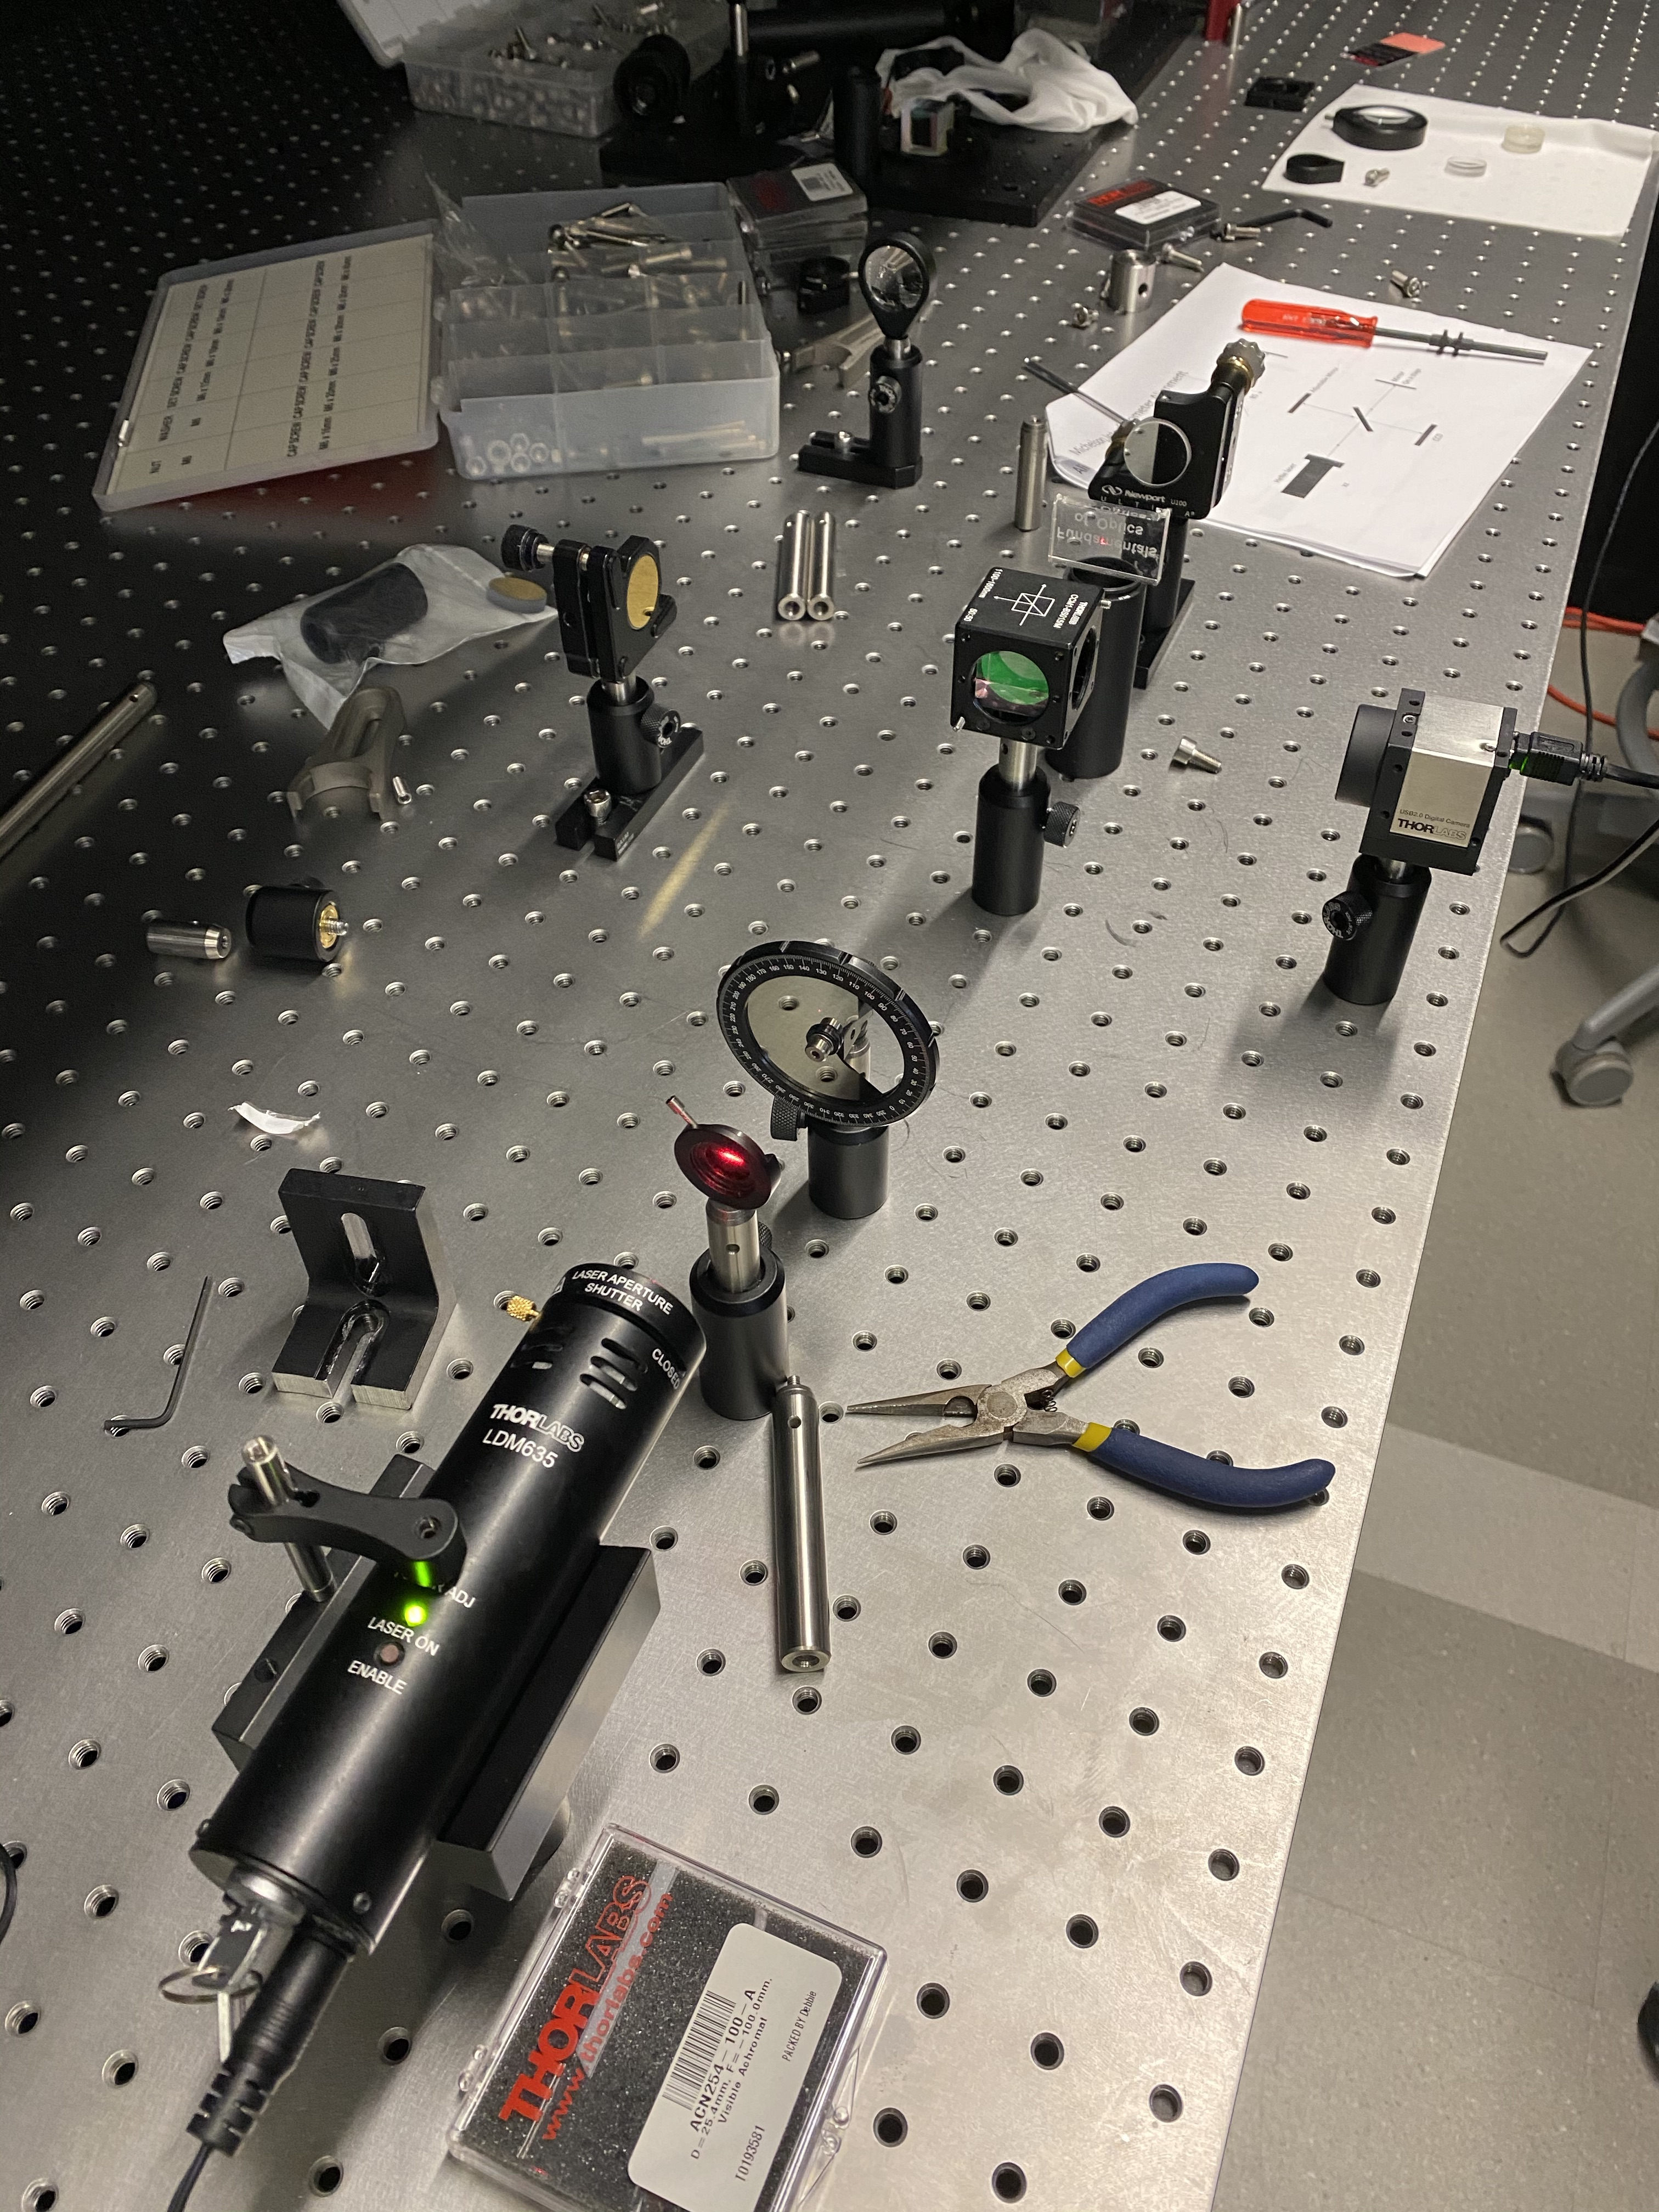
\includegraphics[width=2.5in]{figures/setup3/Michelson_interferometer.png}}
\caption{Setup 3, Michelson Interferometer}
\end{figure}

\begin{figure}\label{fig:5}
\centering\fbox{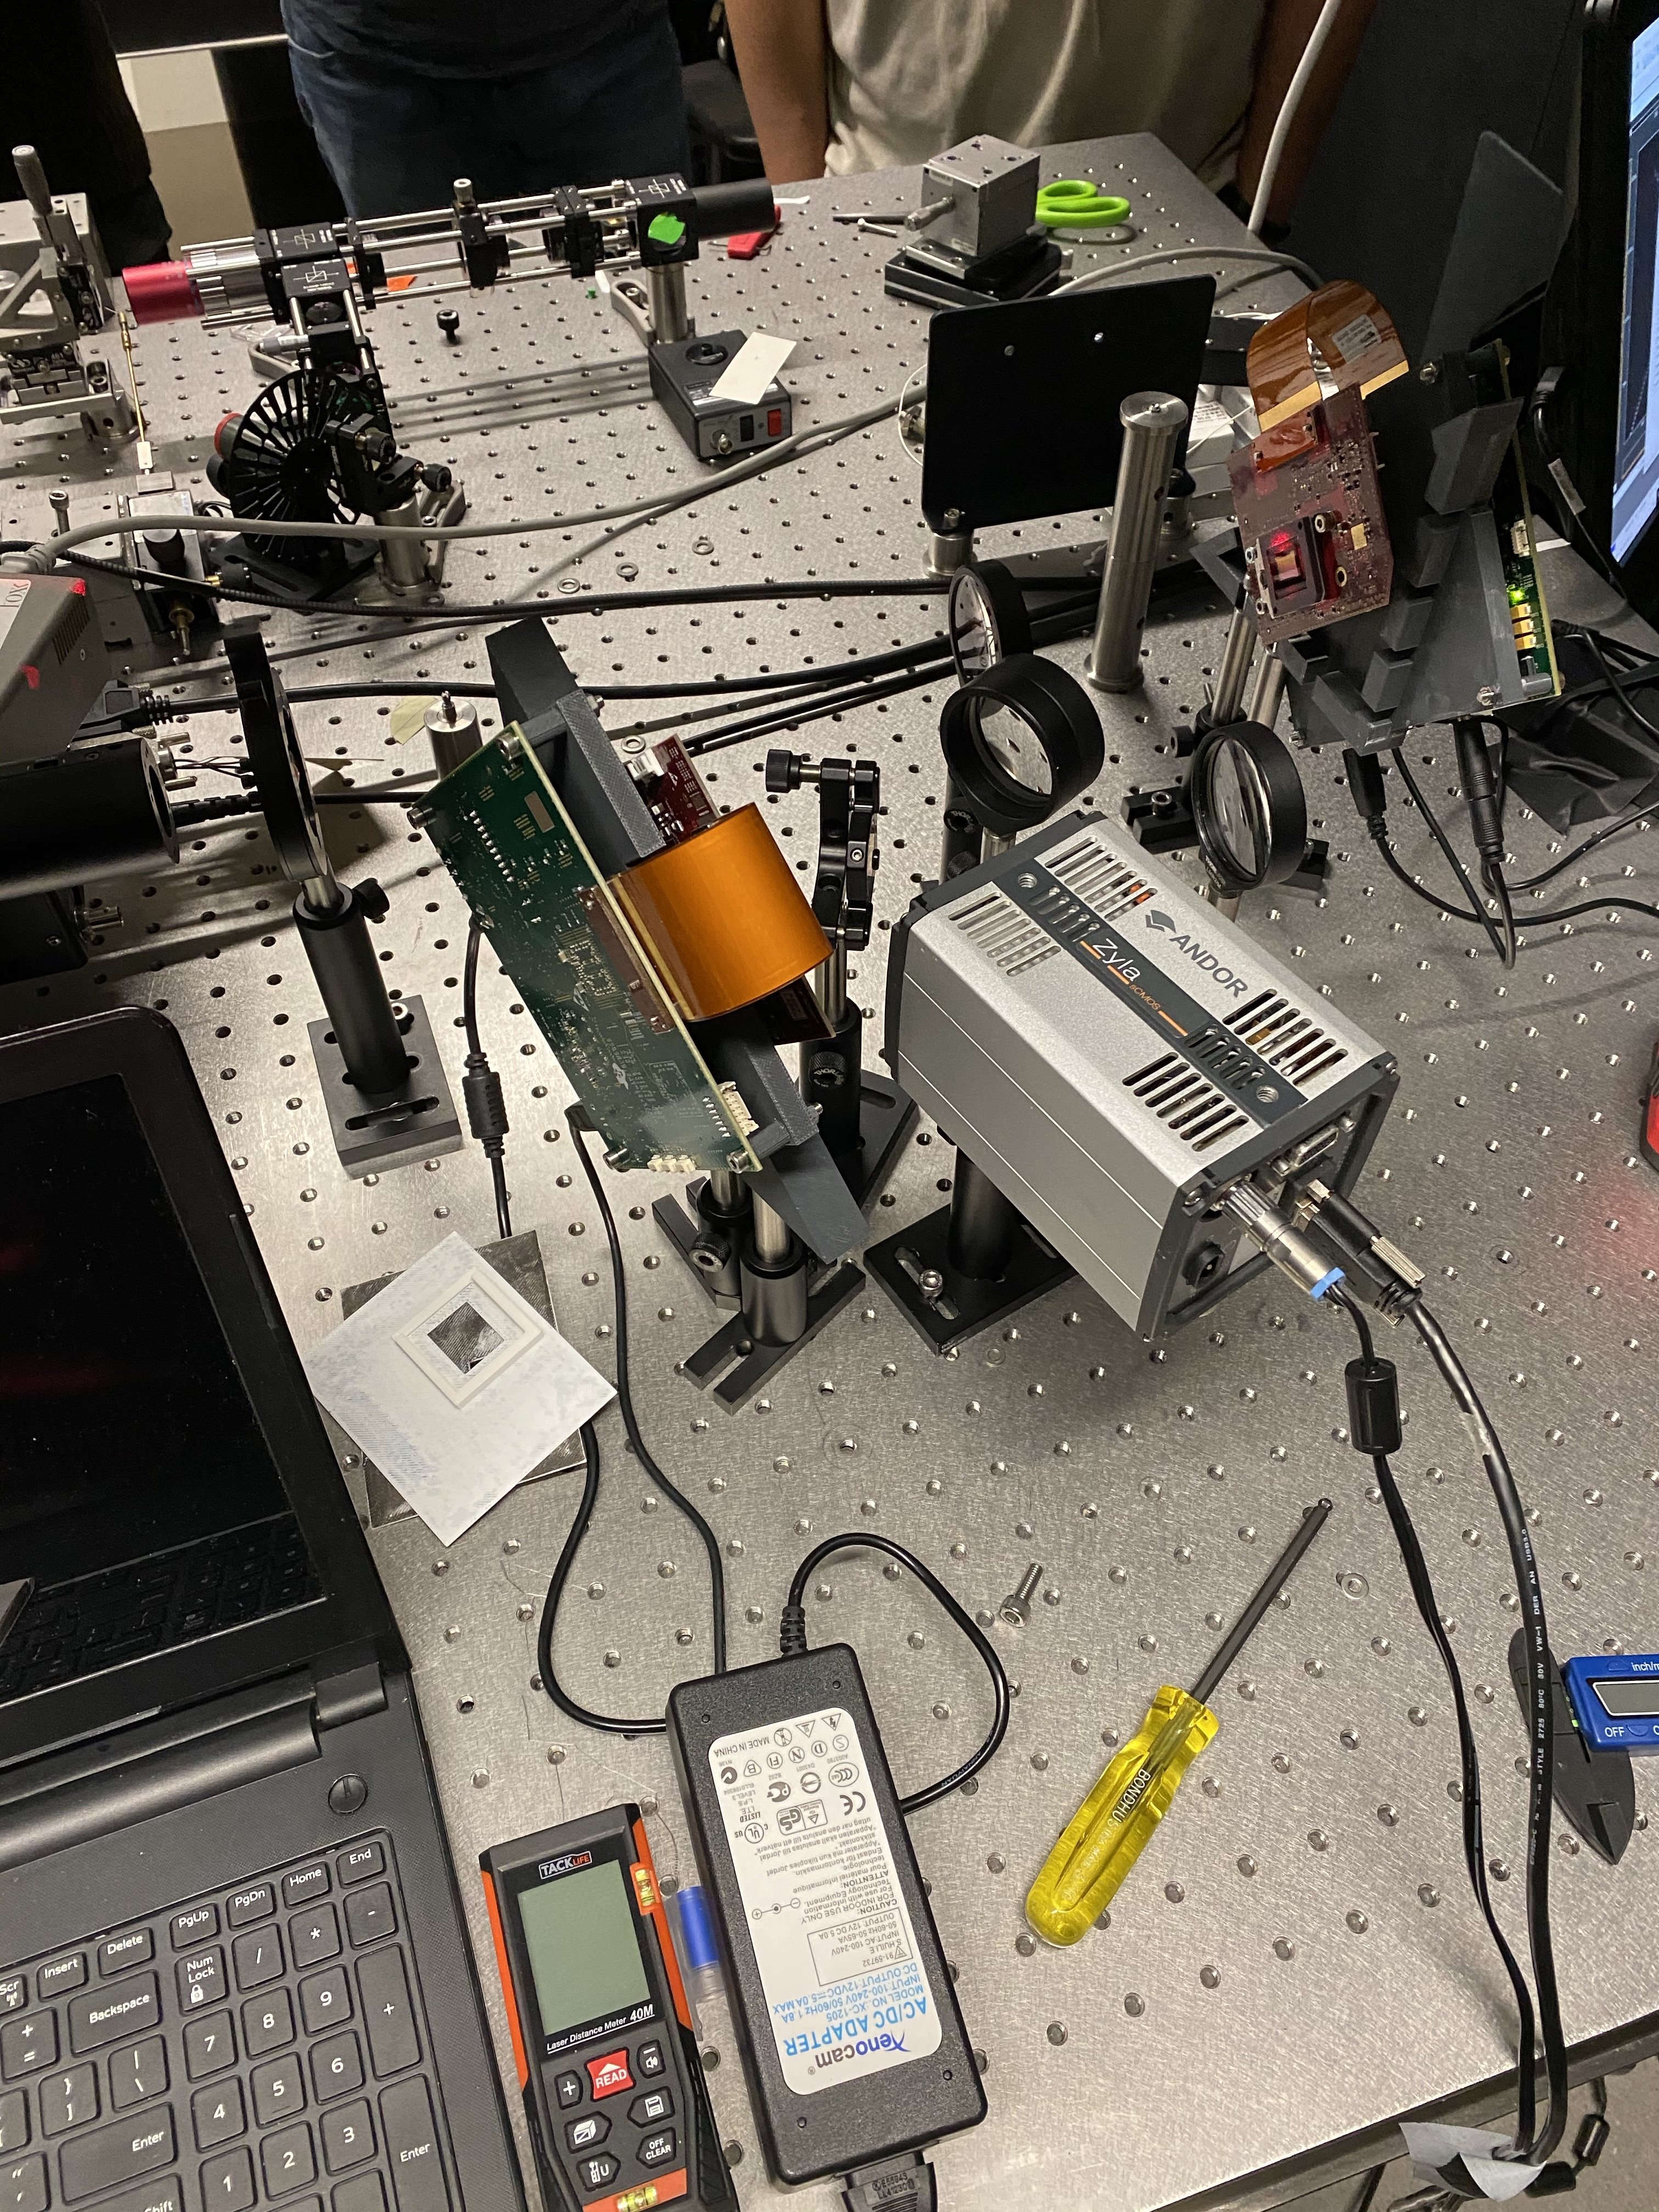
\includegraphics[width=2.5in]{figures/demo/Fourier_Optics.png}}
\caption{Demonstration, Fourier Optics}
\end{figure}

\end{document}